\chapter{Documento de Visão}

\chapter[Relatório Câmera]{Relatório Câmera}
\begin{enumerate}
\item \textbf{Justificativa da escolha}

Para uma melhor análise das condições de tráfego veicular nas rodovias, com o
intuito de projetar um sistema que emite alertas de colisão veicular, fez-se
necessário o acréscimo de uma câmera a qual possibilitasse colher mais informações
do tráfego dos veículos, assim como sua posição na pista, com objetivo de
diminuir os erros de dados do sistema. Para isso foi escolhido uma câmera
com base no sistema anti colisão  Toyota Safety Sense \cite{toyota_safety}, cujo modelo é o AWS650 da 3M.

\item \textbf{Justificativa da câmera AWS650}

Para um bom desenvolvimento do projeto, fez-se necessário uma abrangência maior de dispositivos para coletar informações no ambiente de tráfego do veículo, para que dessa forma obtenha-se redundância de informações com o intuito de evitar falha no sistema  caso algum outro dispositivo falhe. Tais requisitos são:

-  Mudança de faixa do veiculo;

-  Detecção de veículos a frente;

A partir dessas premissas, foi analisado dois sistemas que se destacaram perante os demais existentes, tais sistemas foram:

-Toyota Safety sense;

- AWS650;

\item \textbf{Especificações}
\begin{enumerate}
\item \textbf{Toyota Safety Sense}

Identifica quando o veículo da frente está parado e assim emite um alerta para o condutor de forma que o mesmo possa ter tempo de reação para acionar o sistema de freios ou então o acionamento automático caso o condutor não o acionou quando avisado pelo sistema;

Identifica quando a roda do veiculo muda de faixa da pista, emitindo um alerta sonoro ao condutor;

Suporte de visibilidade no Dispositivo AWS650turna, onde identifica um veiculo vindo no sentido oposto, e posteriormente o sistema altera o farol para farol baixo;

Detecta pedestre na pista e aciona o sistema de freios do automóvel de forma a evitar colisão;

\item \textbf{AWS650}
Mede e calcula em tempo real a distância entre o veiculo e o veiculo que está imediatamente em sua frente, emitindo um alerta sonoro ao condutor caso essa distância seja muito próxima;

Identifica e calcula em tempo real a distância entre as rodas do veiculo e as faixas da esquerda e da direita, emitindo um alerta sonoro ao condutor, mostrando que houve uma mudança de faixa;
\end{enumerate}

\item \textbf{Escolha}

Com base nos itens analisados e nos requisitos do projeto, foi escolhido a câmera AWS650, pois a mesma atende todos os requisitos do projeto na qual será utilizado todas as funções da câmera. Tal escolha foi baseada no sistema  da Toyota Safety Sense, em que não foi escolhido por possuir excesso de funções que não vão ser úteis para o sistema, além de tais funções interferirem no funcionamento do veiculo, como o acionamento dos freios  por exemplo,  onde viola a restrição do projeto no qual diz que o sistema não pode interferir nas funções de funcionamento do veículo.

Segundo a Care Drive \cite{care_drive}, AWS é usado principalmente em estradas, via expressa urbana e outra estrada de alta qualidade, cujo principal objetivo é de auxiliar o condutor a manter-se na pista de forma a evitar acidentes de trânsito causado pela fuga de faixa a qual o mesmo percorre, assim como manter a  distância entre os veículos na pista, evitando assim, colisões frontais. O produto combina identificação de imagem, estimativa de risco e muitas tecnologias de ponta. Quando o veículo ultrapassa a faixa da pista à qual percorre, aproxima-se muito do veículo da frente ou tenta ultrapassar a curta distância, o sistema soa um alarme ao motorista automaticamente para que o mesmo possa corrigir a direção ou aumente a distância entre os veículos.

O sistema AWS apenas tem a função de alertar a segurança ao condutor, cabendo a ele tomar as devidas ações necessárias para corrigir o veículo de forma a manter a segurança, aspecto esse, que atende ao requisito do projeto de não alterar as funções do veículo, apenas oferecer ao condutor a informação.

\begin{figure}[h]
  \centering
  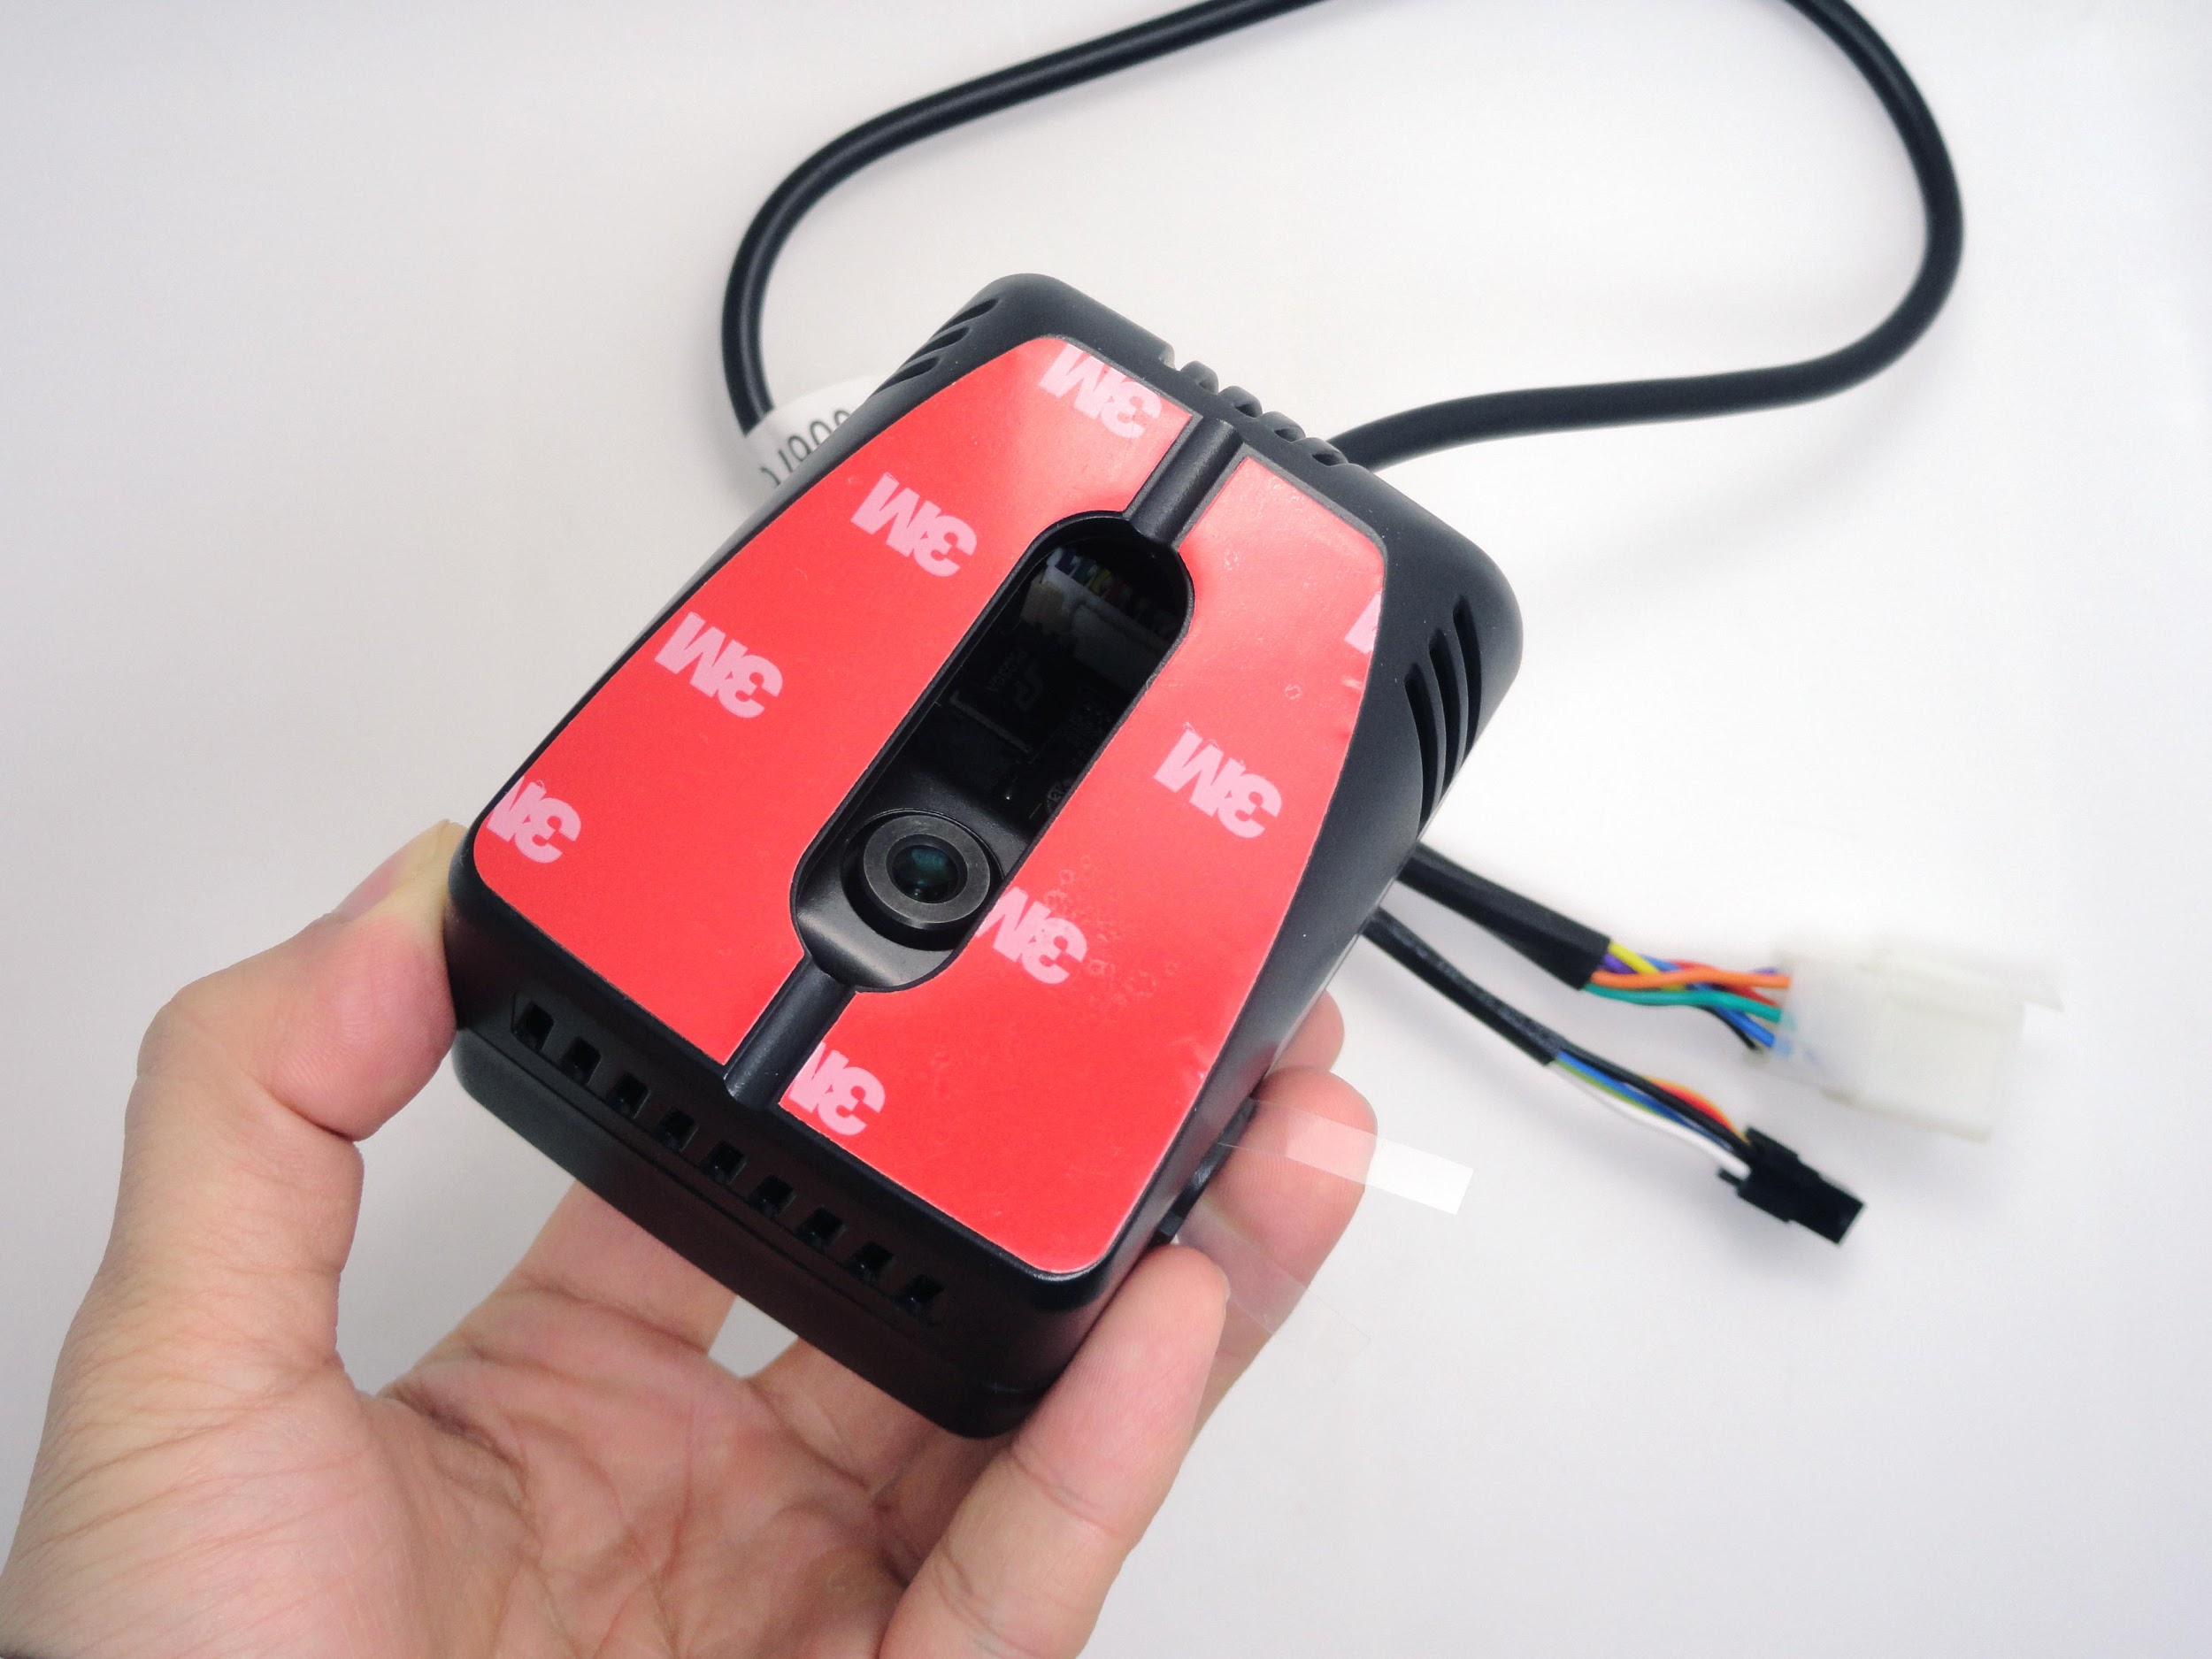
\includegraphics[width=400px, scale=1]{figuras/dispositivo_AWS650}
  \caption{Esquemático do funcionamento do radar}
\label{fig:dispositivo_AWS650}
\end{figure}

\item \textbf{Especificaçoes do AWS650}

A tabela abaixo mostra as especificações do produto:

\begin{table}[ht]
\caption{Especificaçoes do AWS650}
\centering
\begin{tabular}{| l |  p{10cm} |}
\hline
Princípio & aReconhecer e seguir a posição frontal do veículo na faixa pela câmera frontal, calculando em tempo real a distância entre a faixa da direita e a faixa da esquerda e a roda dianteira do veículo.sdf\\
\hline
Condição de alarme & Quando a velocidade do motorista está acima da velocidade permitida da via;

Quando o veículo demonstra não ativar as setas de mudança de faixa;

Quando a roda frontal do veículo excede a faixa da via, ou quando existe a possibilidade de excedê-la.

\\
\hline
Funcionamento do alarme & Quando o produto alertar, enviará o som de alarme "zhi zhi" de imediato, as luzes vermelhas indicativas piscarão, o assento vibrará constantemente. A intenção do condutor em realizar a mudança de faixa com o acionamento e o desligamento da seta quando retornar à sua faixa original, o alarme parará de indicar que o veículo terminou a mudança de faixa.

A função de vibração do alarme funcionará apenas quando o motorista comprar o assento vibratório, caso contrário, funcionará apenas com as funções dos sons e das luzes indicativas.\\

\hline
Luz Amarela & Não alcance a velocidade máxima da via;

Não reconhece a faixa de direção;

O motorista freia ou ativa a seta sinalizadora;

Câmera com problemas (pisca-pisca).\\
\hline
Luz Vermelha & aviso de alarme (pisca-pisca).\\
\hline
Luz Verde & Reconhece e segue a faixa de direção;

direção segura .\\
\hline
Luz Verde & Reconhece e segue a faixa de direção;

Direção segura.\\
\hline
Falha do Sistema & 1. Chuva forte, Forte neblina, condições climáticas como neve/nevascas, visibilidade horizontal é menor do que 1km.

2. A sinalização horizontal da faixa é fraca ou não satisfaz os parâmetros do GB5768.

3. Não satisfaz a condição ambiental do GBT26773-2011.
\\
\hline
\end{tabular}
\label{table:funcionamento_aws650}
\end{table}

\begin{figure}[h]
  \centering
  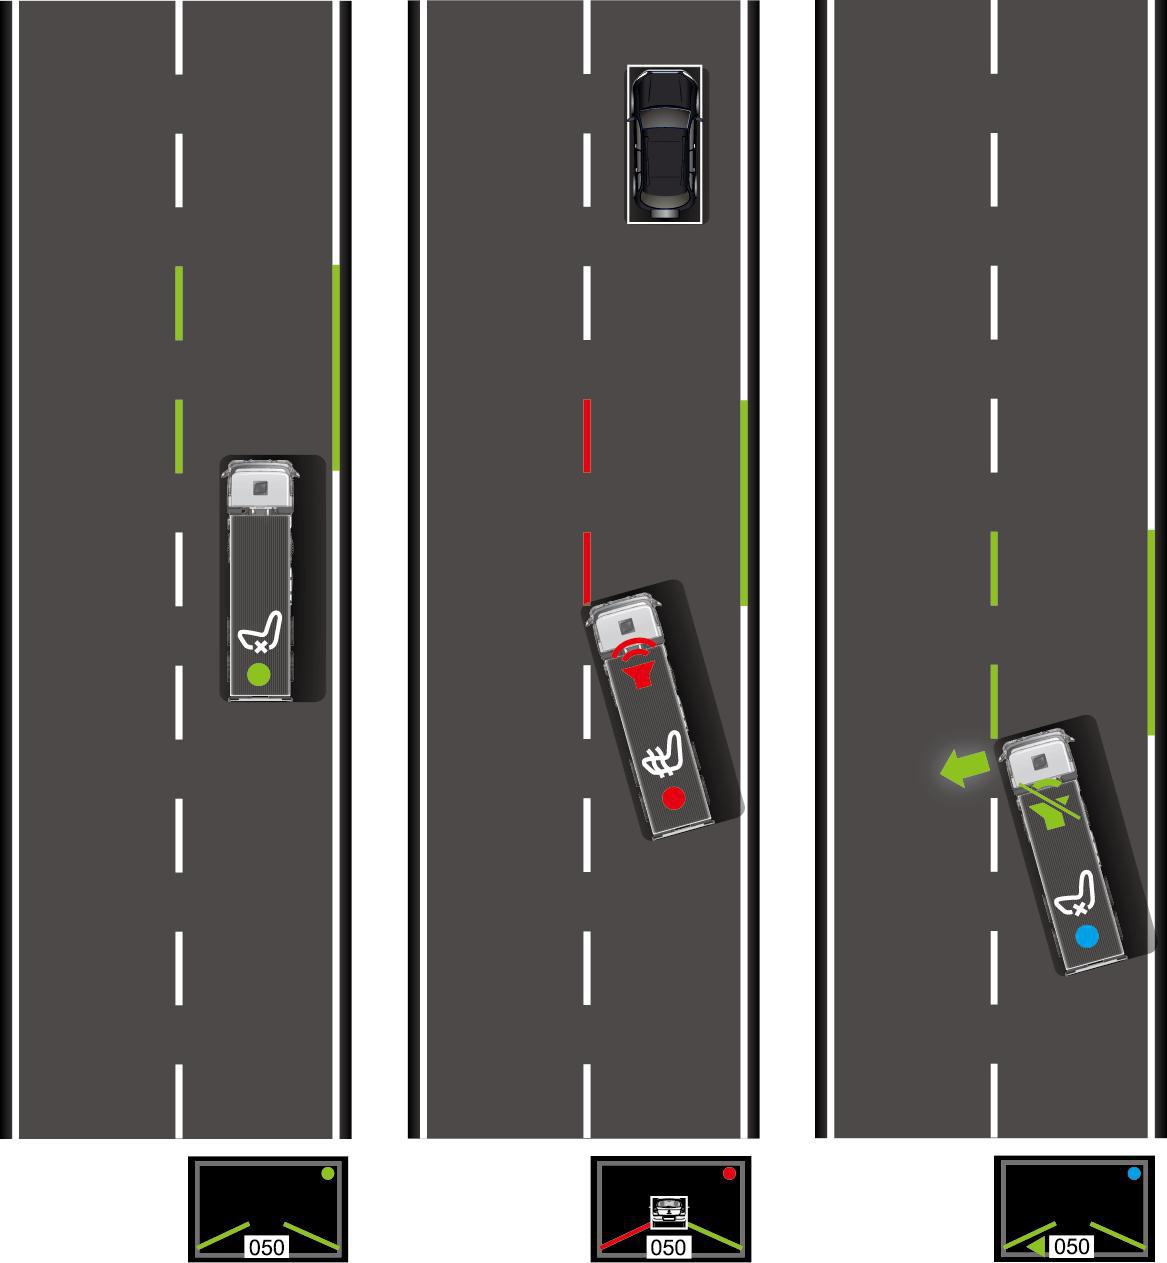
\includegraphics[width=400px, scale=1]{figuras/aviso_mudanca_faixa}
  \caption{Ilustração do sistema de aviso de mudança de faixa}
\label{fig:aviso_mudanca_faixa}
\end{figure}

\item \textbf{Aviso Dianteiro de Colisão}

Nesse quesito o sistema funciona de acordo com a tabela \ref{table:aviso_dianteiro} abaixo:

Sistema de alerta anticolisão frontal (FCW)

Quando o veículo está muito próximo do veículo da frente ou tem um perigo de colisão, será fornecido o alarme sonoro para avisar ao motorista de forma que o mesmo tome ações a fim de evitar que o acidente aconteça, reduzindo a perda do acidente.

\begin{table}[ht]
\caption{Aviso dianteiro de colisão do AWS650}
\centering
\begin{tabular}{| l |  p{10cm} |}
\hline
Princípio & Reconhece e segue de perto o veículo da frente pela câmera frontal, calculando em tempo real a distância entre os dois veículos e o tempo de reação ao perigo. \\
\hline
Condição de alarme & A velocidade do motorista alcança a velocidade máxima da via;
A distância de segurança é menor que 1.3s ou o tempo de reação ao perigo é menor que 2.7s (50km/h quando dirigindo, a distância de segurança é de aproximadamente 18 metros).
\\
\hline
Funcionamento do Alarme & Quando o produto alerta, enviará o som "di di di" de imediato;

As luzes indicativas piscarão, o assento vibrará continuamente em intervalos. Quanto maior a velocidade do veículo menor será o intervalo de vibração;

Maior perigo para a distância entre os dois veículos, o tempo de vibração será mais longo e contínuo.

A função vibratória do alarme só funcionará quando o motorista comprar o assento vibratório, caso contrário funcionará somente com as funções de som e luzes indicativas.

A intenção do motorista de frear para controlar a velocidade de condução;

A distância entre os dois veículos é maior do que a distância de segurança, o alarme parará.
 \\
\hline
Luz amarela & Não alcança a velocidade máxima da via, não reconhece o veículo; o motorista freia ou faz o sinal de mudança de faixa, problema com a câmera (pisca-pisca).
 \\
\hline
Luz Vermelha & Aviso de alarme (pisca-pisca). \\
\hline
Falha do Sistema & 1. Chuva forte, Forte neblina, condições climáticas como neve/nevascas, visibilidade horizontal é menor do que 1km.

2.   Não satisfaz a condição ambiental do GBT26773-2011. \\
\hline
\end{tabular}
\label{table:aviso_dianteiro}
\end{table}


\begin{figure}[h]
  \centering
  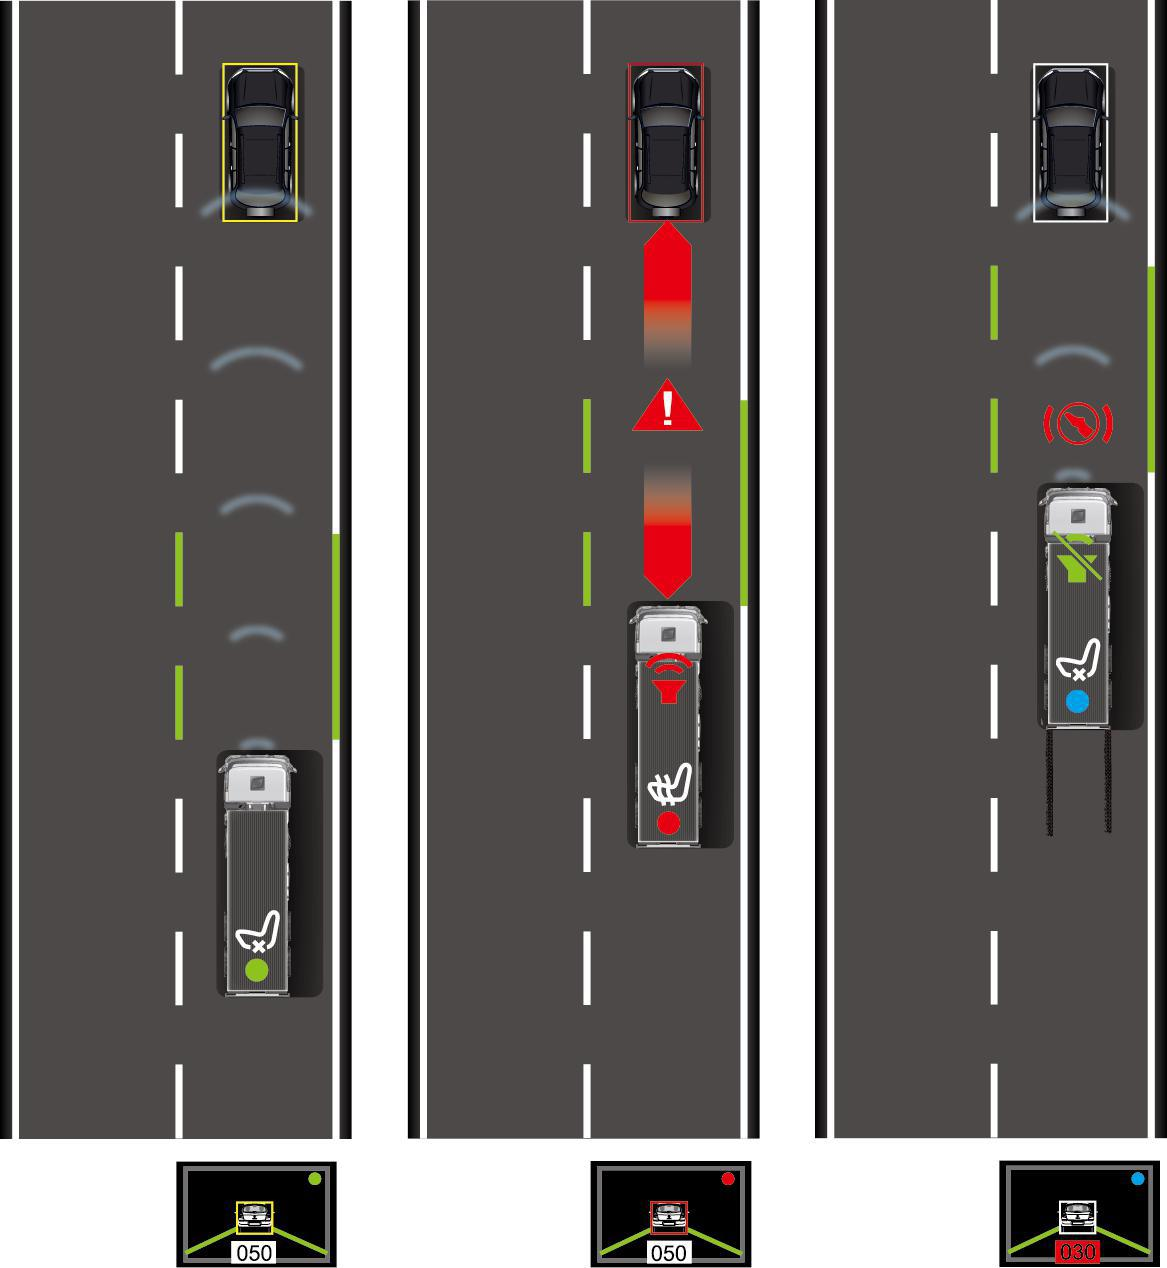
\includegraphics[width=400px, scale=1]{figuras/funcionamento_sistema_frontal}
  \caption{ Ilustração do funcionamento do sistema de alerta anti colisão frontal}
\label{fig:funcionamento_sistema_frontal}
\end{figure}

\item \textbf{Função de saída de video}
As funções de video do sistema AWS650 estão descritos nas imagens \ref{fig:visao_camera} e \ref{fig:visao_camera2}, onde mostra como as imagens são processadas em tempo real.


\begin{figure}[h]
  \centering
  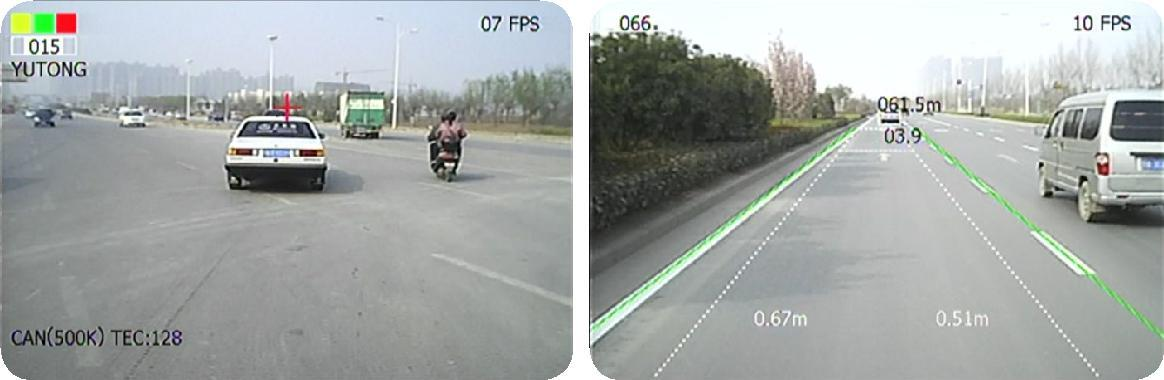
\includegraphics[width=400px, scale=1]{figuras/visao_camera}
  \caption{Ilustração do funcionamento do processamento de video do AWS650}
\label{fig:visao_camera}
\end{figure}

\begin{figure}[h]
  \centering
  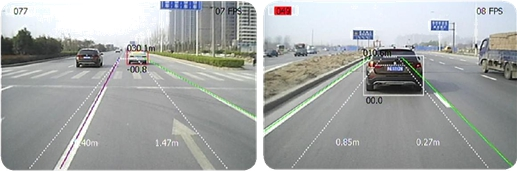
\includegraphics[width=400px, scale=1]{figuras/visao_camera2}
  \caption{Ilustração 2 do funcionamento do processamento de video do AWS650}
\label{fig:visao_camera2}
\end{figure}

\item \textbf{Instalação}
Para uma melhor visibilidade do AWS650, o dispositivo deve ser acoplado no para brisas do automóvel, onde não pode haver nenhum tipo de sujeira no dispositivo que possa impedir sua visão, dessa forma o mesmo terá uma maior área de visibilidade da pista para realizar a varredura. A disposição do dispositivo no centro do para brisas se dá também para que ele não prejudique a visão do condutor.

De modo que o dispositivo tenha um correto funcionamento, deve-se seguir corretamente o processo de calibragem da câmera ao automóvel à qual será instalado, tal procedimento está melhor illustrado na figura \ref{fig:instalacao_camera}:


\begin{figure}[h]
  \centering
  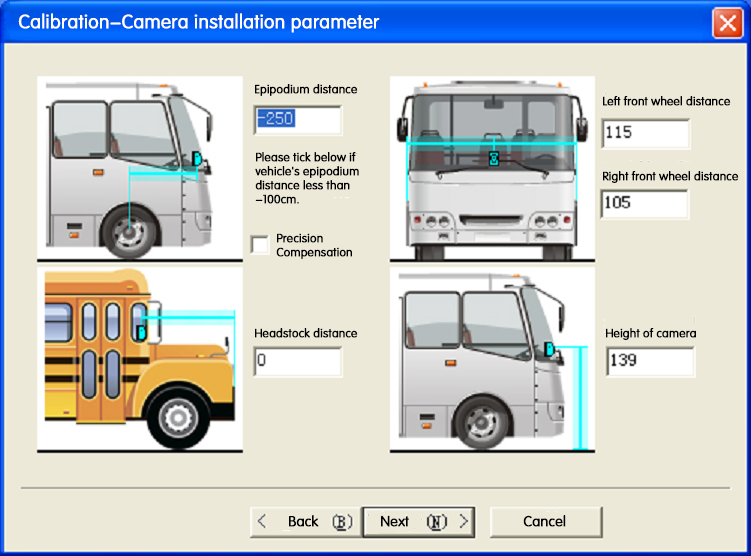
\includegraphics[width=400px, scale=1]{figuras/instalacao_camera}
  \caption{Ilustração da calibragem do dispositivo AWS650 no automóvel}
\label{fig:instalacao_camera}
\end{figure}
\end{enumerate}
